\mysubsection{Architecture orientée service (SOA)}

\ifbook{
  \mysubsubsection{WebServices}
}


\ifslide{
  \begin{frame}{Web Service}
    \begin{block}{Qu'est qu'un \textit{Web Service}}
      \begin{itemize}
        \item même concept que le Web mais appliqué la communication entre machine
        \item donc moins orienté "lecture" (plus d'opération d'écriture)
        \item plus "dynamic"
        \item support des environements hétérogènes
      \end{itemize}
    \end{block}
  \end{frame}

  \begin{frame}{Web Service}
    \begin{block}{Indépendance du \textit{End Point}}
      \begin{itemize}
        \item traitement réparti
        \item maintenance du noeud indépendante
        \item négociation de protocole
        \item couplage lâche
      \end{itemize}
    \end{block}
  \end{frame}

  \begin{frame}{Web Service}
    \begin{block}{Composition de protocole}
      \begin{itemize}
        \item architecture modulaire
        \item complexité géré par les outils
        \item extensibilité apporté par XML
      \end{itemize}
    \end{block}

    \begin{center}
      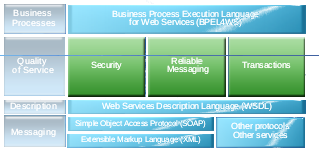
\includegraphics[scale=0.8]{img/web-services.png}
    \end{center}

  \end{frame}

  \begin{frame}{Web Service}
    \begin{center}
      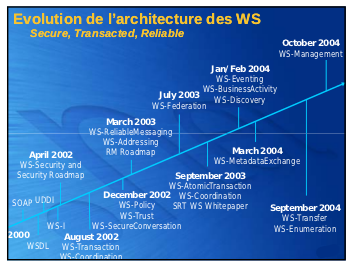
\includegraphics[scale=0.8]{img/ws-star.png}
    \end{center}
  \end{frame}

  \begin{frame}
    \begin{block}{MOM et RPC... en WS !}
      \begin{itemize}
        \item XML-RPC
        \item publish/subscribe
        \item pièce jointe
      \end{itemize}
    \end{block}

    \begin{block}{Indépendance du transport}
      \begin{itemize}
        \item HTTP
        \item TCP
        \item Binaire !
      \end{itemize}
    \end{block}
  \end{frame}

  \begin{frame}
    \begin{block}{Mais aussi...}
      \begin{itemize}
        \item transaction
        \item sécurité
        \item ...
      \end{itemize}
    \end{block}

    \begin{block}{Découverte de Service et Annuaire}
      \begin{itemize}
        \item UDDI
        \item WS-Discovery
      \end{itemize}
    \end{block}
  \end{frame}
}


\ifbook{
  \mysubsubsection{SOA et Bus logiciel (ESB)}
}


\ifslide{

  \begin{frame}
    \begin{block}{SOA}
      \begin{itemize}
        \item architecure
        \item \textit{loose coupling}
        \item fonctionnement par contrat
      \end{itemize}
    \end{block}

    \begin{block}{ESB}
      \begin{itemize}
        \item orchestration
        \item analogue à un Bus électronique
      \end{itemize}
    \end{block}
  \end{frame}

  \begin{frame}{ESB}
    \begin{center}
      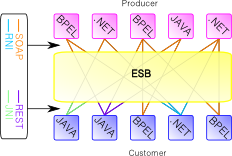
\includegraphics[scale=1]{img/esb.png}
    \end{center}
  \end{frame}


}

\mysubsection{ETL, EAI et autres middlewares}
